\documentclass[11pt,a4paper,oneside]{report}             % Single-side
%\documentclass[11pt,a4paper,twoside,openright]{report}  % Duplex

%\PassOptionsToPackage{chapternumber=Huordinal}{magyar.ldf}
\usepackage{t1enc}
\usepackage[utf8]{inputenc}
\usepackage[english,magyar]{babel}
\usepackage{amsmath}
\usepackage{amssymb}
\usepackage{enumerate}
\usepackage[thmmarks]{ntheorem}
\usepackage{graphics}
\usepackage{epsfig}
\usepackage{listings}
\usepackage{color}
%\usepackage{fancyhdr}
\usepackage{lastpage}
\usepackage{anysize}
\usepackage{sectsty}
\usepackage{setspace}  % Ettol a tablazatok, abrak, labjegyzetek maradnak 1-es sorkozzel!
\usepackage[hang]{caption}
\usepackage{url}								%For URL-s
\usepackage[headheight=56pt]{geometry}			%For the heading gap


%MATHEMATICAL EXPRESSIONS
\usepackage{bm}									%Bolding
\usepackage[scaled=0.85]{beramono}				%for bolding

%TABLES, TABULATING, DRAWING
\usepackage{array}
\usepackage{tabu}
\usepackage{mdframed}
\usepackage{multirow}
\usepackage{tabularx}
\usepackage{tikz}								%For drawing see --
\usepackage{stuki}								%For struktogramms see --
\usepackage{hyperref}

\usetikzlibrary[shadows]

%--------------------------------------------------------------------------------------
% Main variables
%--------------------------------------------------------------------------------------
\newcommand{\szerzo}{Hajnal Máté}
\newcommand{\palyazok}{Szedmák Bálint \& Hajnal Máté}
\newcommand{\cim}{BME-VIK \& ELTE PPK Gólyabál pályázat \\ Programozás beadandó}
\newcommand{\doktipus}{Palyazat}
%--------------------------------------------------------------------------------------
% Page layout setup
%--------------------------------------------------------------------------------------
% we need to redefine the pagestyle plain
% another possibility is to use the body of this command without \fancypagestyle
% and use \pagestyle{fancy} but in that case the special pages
% (like the ToC, the References, and the Chapter pages)remain in plane style

\pagestyle{plain}
%\setlength{\parindent}{0pt} % áttekinthetõbb, angol nyelvû dokumentumokban jellemzõ
%\setlength{\parskip}{8pt plus 3pt minus 3pt} % áttekinthetõbb, angol nyelvû dokumentumokban jellemzõ
\setlength{\parindent}{12pt} % magyar nyelvû dokumentumokban jellemzõ
\setlength{\parskip}{0pt}    % magyar nyelvû dokumentumokban jellemzõ

\marginsize{35mm}{25mm}{15mm}{15mm} % anysize package
\setcounter{secnumdepth}{0}
\sectionfont{\large\upshape\bfseries}
\setcounter{secnumdepth}{2}
\singlespacing
\frenchspacing

%--------------------------------------------------------------------------------------
% Set up listings
%--------------------------------------------------------------------------------------
\lstset{
	basicstyle=\scriptsize\ttfamily, % print whole listing small
	keywordstyle=\color{black}\bfseries\underbar, % underlined bold black keywords
	identifierstyle=, 					% nothing happens
	commentstyle=\color{white}, % white comments
	stringstyle=\scriptsize\sffamily, 			% typewriter type for strings
	showstringspaces=false,     % no special string spaces
	aboveskip=3pt,
	belowskip=3pt,
	columns=fixed,
	backgroundcolor=\color{lightgray},
} 		
\def\lstlistingname{lista}	

%--------------------------------------------------------------------------------------
%	Some new commands and declarations
%--------------------------------------------------------------------------------------
\newcommand{\code}[1]{{\upshape\ttfamily\scriptsize\indent #1}}

% define references
\newcommand{\figref}[1]{\ref{fig:#1}.}
\renewcommand{\eqref}[1]{(\ref{eq:#1})}
\newcommand{\listref}[1]{\ref{listing:#1}.}
\newcommand{\sectref}[1]{\ref{sect:#1}}
\newcommand{\tabref}[1]{\ref{tab:#1}.}

\DeclareMathOperator*{\argmax}{arg\,max}
%\DeclareMathOperator*[1]{\floor}{arg\,max}
\DeclareMathOperator{\sign}{sgn}
\DeclareMathOperator{\rot}{rot}
\definecolor{lightgray}{rgb}{0.95,0.95,0.95}

\author{\szerzo}
\title{\title}
\includeonly{
	titlepage,%
	chapter2,%
	acknowledgement,%
}
%--------------------------------------------------------------------------------------
%	Setup captions
%--------------------------------------------------------------------------------------
\captionsetup[figure]{
%labelsep=none,
%font={footnotesize,it},
%justification=justified,
width=.75\textwidth,
aboveskip=10pt}

\renewcommand{\captionlabelfont}{\small\bf}
\renewcommand{\captionfont}{\footnotesize\it}


%--------------------------------------------------------------------------------------
%	Setup hyperref package
%--------------------------------------------------------------------------------------
\hypersetup{
    unicode=true,              % non-Latin characters in Acrobat’s bookmarks
    pdftitle={\cim},           % title
    pdfauthor={\szerzo},       % author
    pdfsubject={\doktipus},    % subject of the document
    pdfcreator={\szerzo},      % creator of the document
    pdfproducer={Producer},    % producer of the document
    pdfkeywords={keywords},    % list of keywords
    pdfnewwindow=true,         % links in new window
    colorlinks=true,           % false: boxed links; true: colored links
    linkcolor=black,           % color of internal links
    citecolor=black,           % color of links to bibliography
    filecolor=black,           % color of file links
    urlcolor=black             % color of external links
}

%--------------------------------------------------------------------------------------
% Table of contents and the main text
%--------------------------------------------------------------------------------------
\begin{document}
\onehalfspacing
%--------------------------------------------------------------------------------------
%	The title page
%--------------------------------------------------------------------------------------
\begin{titlepage}
\begin{center}
\includegraphics[width=150mm,keepaspectratio]{figures/eiffel_tower.png}\\
\vspace{0.3cm}
\textbf{Budapesti Mûszaki és Gazdaságtudományi Egyetem}\\
\textmd{Villamosmérnöki és Informatikai Kar}\\
\textmd{\viktanszek}\\[5cm]

\vspace{0.4cm}
{\huge \bfseries \vikcim}\\[0.8cm]
\vspace{0.5cm}
\textsc{\Large \vikdoktipus}\\[4cm]

\begin{tabular}{cc}
 \makebox[7cm]{\emph{Készítette}} & \makebox[7cm]{\emph{Konzulens}} \\
 \makebox[7cm]{\vikszerzo} & \makebox[7cm]{\vikkonzulens}
\end{tabular}

\vfill
{\large \today}
\end{center}
\end{titlepage}



\tableofcontents\vfill
%----------------------------------------------------------------------------
\chapter{Programozás házi feladat}\label{sect:ProgHF}
%----------------------------------------------------------------------------

%----------------------------------------------------------------------------
\section{Feladat}
%----------------------------------------------------------------------------

\textit{Egy étteremben a pincérek által felvett rendeléseket egy szekvenciális input fájlban tartják nyilván az ételek neve, azon belül a rendelések időpontja szerint rendezett formában. Feltehetjük, hogy a fájl nem üres. A tárolt adatok: a rendelt étel neve, a rendelés időpontja, rendelt adagok száma, egy adag ára. Melyik étel hozta az étteremnek a legtöbb bevételt (összesített darab*egységár)?}\\

%----------------------------------------------------------------------------
\section{Specifikáció}
%----------------------------------------------------------------------------
A feladat állapottere többféleképpen felírható
% A feladat állapottere
\begin{flalign*}
	A=(f:Infile(&\mathbb{K}),~cout:Outfile(\mathbb{K}))\\
	A=(f:Infile(&Sor),~cout:Outfile(Sor))\\
	A=(f:Infile(&Rendeles), cout:String)\\
	&Rendeles=\textbf{rec}(nev:String, ido:\mathbb{N}, adag:\mathbb{N}, ar:\mathbb{N})\\
\end{flalign*}
Számunkra a legideálisabb már egy olyan felsorolón dolgozni, ami rendelés nevű rekordokat dolgozni, melyek a rendelések nevét és hozzájuk tartozó bevételeket tartalmazzák. Erre a felsorolóra kell nekünk egy maximum keresést írni.\\
% Összegzés, összefűzés
A maximumkeresés:
\begin{flalign*}
	&A=(t:Enor(Rendeles),~cout:String,~max:\mathbb{N},~elem:Rendeles)\\
	&\hspace{25mm}Rendeles=\textbf{rec}(nev:String, bevetel:\mathbb{N})\\
	&Ef=(t=t'~\wedge~|t'|>0~\wedge~t.azon\uparrow)\\
	&Uf=((max,~elem)=\max_{e\in t'}{(e.bevetel)}~\wedge~cout=elem.nev)\\
\end{flalign*}

%----------------------------------------------------------------------------
\section{Absztrakt program}
%----------------------------------------------------------------------------
\begin{center}
\begin{tabular}{|lll|}
	\hline
	\multicolumn{3}{|c|}{\textbf{Maximum~keresés}}\\
	\hline
	t & $\sim$ & \textit{Rendelések bevételeivel való felsorolója}\\
	+,0 & $\sim$~ & \textit{+,0}\\
	f(e) & $\sim$ & \textit{e.bevetel}\\
	\hline
\end{tabular}
\end{center}

\noindent\hfill
	\begin{stuki}[12cm]
		\stm{t.First()}
		\stm{max,~elem:=t.Current().bevetel,~t.Current()}
		\stm{t.Next()}
		\begin{WHILE}{4}{\stm{\lnot t.End()}}
			\begin{IF}[70]{2}{\stm{t.Current().bevetel>max}}
				\stm{max,~elem:=t.Current().bevetel,~t.Current()}
			\ELSE
				\stm{SKIP}
			\end{IF}
			\stm{t.Next()}
		\end{WHILE}
		\stm{cout:=elem.nev}
	\end{stuki}
\vspace{5mm}
\textbf{Rendelések bevételeivel való felsorolója:}
\vspace{5mm}\\
	\begin{tabular}{|l|l|}
		\hline
		\textit{enor(Rendeles)}& \textit{First(),Next(),Current(),End()}\\
		\hline
		\textit{f:Infile(nev:String,ido:$\mathbb{N}$,adag:$\mathbb{N}$,ar:$\mathbb{N}$) }& \textit{First()$\sim$ st, $akt_f$, f:read;Next()}\\
		\textit{st:Status} & \textit{Next()$\sim$ lsd.külön}\\
		\textit{elso:String} & \textit{Current()$\sim$ akt}\\
		\textit{akt:Rendeles} & \textit{End() $\sim$ st=abnorm}\\
		\textit{$akt_f$:rec(nev:String,ido:$\mathbb{N}$,adag:$\mathbb{N}$,ar:$\mathbb{N}$)} & \\
		\hline
	\end{tabular}
\vspace{5mm}\\
\indent A First művelettel beolvastunk a szekvenciális input fájlunkból egy rendelés elemet, melyet az $akt_f$ rekordban tárolunk. A beolvasás sikerességét a státusz jelzés jelzi nekünk.\\
\indent A Next művelet több feladatot, kell ellásson. Addig kell olvasson a szekvenciális input fájlból, amíg a rendelés nevek megegyeznek, vagy véget nem ér a fájl. Ehhez először egy elso nevű változóban eltároljuk az aktuális rendelés nevét, továbbá ehhez hasonlóan egy akt nevű változóban eltároljuk a szükséges rendelés paramétereket, (név és bevétel=adag*ár). Az összegzést, úgy valósítjuk meg, hogy az $akt_f$-be beolvasott input fájl értékek segítségével (az adag*ár értékekkel) az aktuális felsoroló elem $akt$ bevétel nevű változóját növelgetjük. A ciklus akkor marad abba, ha a beolvasás nem sikerült, vagy új rendelésünk van.
\begin{flalign*}	
	&A^{Next}=(f:Infile(nev:String,ido:\mathbb{N},adag:\mathbb{N},ar:\mathbb{N}),elso:String,st:Status,\\
	&\hspace{30mm}act_f:rec(nev:String,ido:\mathbb{N},adag:\mathbb{N},ar:\mathbb{N}),akt:Rendeles)\\
	&Ef^{Next}=(f=f^1~\wedge~st=st^1~\wedge~akt_f=akt_f^1)\\
	&Uf^{Next}=((st=norm\rightarrow elso=akt_f^1.nev\\
	&\hspace{30mm}\wedge~akt.bevetel^2=0)~\wedge~\\
	&(st^2,{akt_f}^2,f^2)=((akt.nev,akt.bevetel)=\sum\limits_{akt_f\in {akt_f}^1,f^1}^{elso=akt_f.nev \wedge st=norm}{(akt_f.nev,} \\
	&\hspace{10mm}akt.bevetel+akt_f.adag*akt_f.ar)\\
\end{flalign*}

\begin{center}
\begin{tabular}{|lll|}
	\hline
	\multicolumn{3}{|c|}{\textbf{Összegzés}}\\
	\hline
	+,0 & $\sim$~ & \textit{+,0}\\
	f(e) & $\sim$ & $akt.bevetel:(akt_f.adag*akt_f.ar)$ \\
	\hline
\end{tabular}
\end{center}

\noindent\hfill
\begin{stuki}[12cm]
	\begin{IF}[70]{2}{\stm{st=norm}}
		\stm{elso,akt.nev,akt.bevetel=\\
		akt_f.nev,0}
	\ELSE
		\stm{SKIP}
	\end{IF}
	\begin{WHILE}{2}{\stm{elso=akt_f.nev \wedge st=norm}}		
		\stm{akt.nev,akt.bevetel:=akt_f.nev,akt.bevetel+akt_f.adag*akt_f.ar}
		\stm{st,akt_f,f:read}
	\end{WHILE}
\end{stuki}


%----------------------------------------------------------------------------
\section{Implementáció}
%----------------------------------------------------------------------------
Program váz: A program több állományból áll: \texttt{etterem.cpp, enor.h, enor.cpp}
\begin{center}
\begin{tabular} {|l|l|l|}
	\hline
	\textbf{etterem.cpp} & \textbf{enor.h} & \textbf{enor.cpp} \\
	\hline
	\texttt{int main()} & \texttt{struct} $Akt_f$ & \texttt{Enor::Read()} \\
	& \texttt{struct Rendeles} & \texttt{Enor::Enor()} \\
	& \texttt{Enor()} & \texttt{Enor::Next()} \\
	& \texttt{void First()} & \\
	& \texttt{void Next()} & \\
	& \texttt{Rendeles Current()} & \\
	& \texttt{bool End()} & \\
	\hline
\end{tabular}
\end{center}
A függvények kapcsolódási szerkezete:\\
\begin{center}
	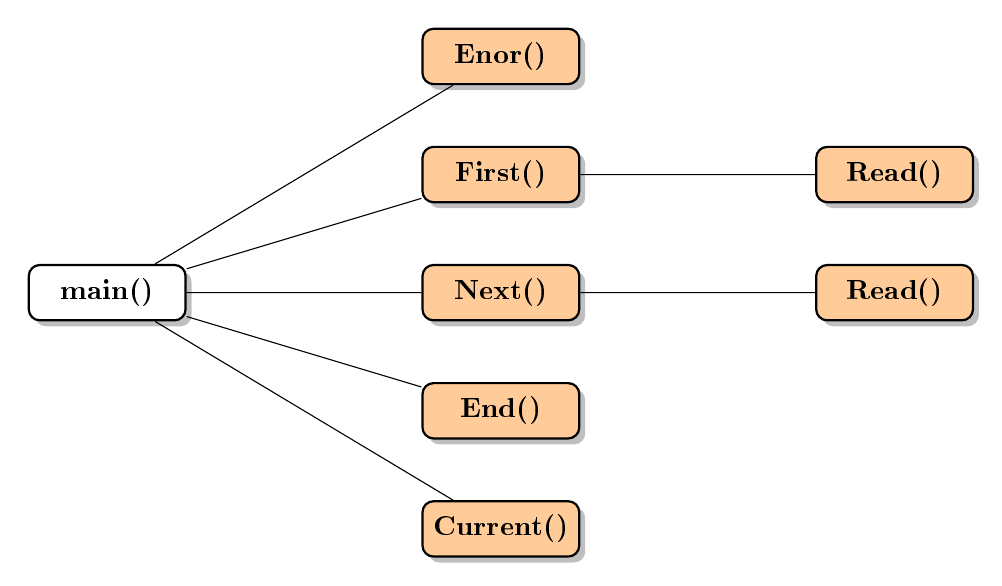
\begin{tikzpicture}
		[grow=right, align=center, root/.style={rectangle, draw=black, thick, drop shadow, fill=white, text width=5em, rounded corners, minimum height=2em}, leaf/.style={rectangle, draw=black, thick, drop shadow, fill=orange!40, text width=5em, rounded corners, minimum height=2em}, level distance=5cm];
		\node [root] (main) {\textbf{main()}}
			child {node [leaf] (current) {\textbf{Current()}}}
			child {node [leaf] (end) {\textbf{End()}}}
			child {node [leaf] (next) {\textbf{Next()}}
				child {node [leaf] (readb) {\textbf{Read()}}}
			}
			child {node [leaf] (first) {\textbf{First()}}
				child {node [leaf] (reada) {\textbf{Read()}}}
			}				
			child {node [leaf] (enor) {\textbf{Enor()}}};
	\end{tikzpicture}\vspace{2mm}\\
\end{center}
A felsoroló osztálya:\\
	\begin{mdframed}
		\texttt{
		\begin{tabbing}
		\hspace{1cm}\=\textbf{class} Enor\{ \+\\
		    \hspace{1cm}\=\textbf{private:} \+\\
		        \hspace{1cm}\=std::ifstream f;\+\\
		        Status st;\\
		        Rendeles akt;\\
		        $Akt_f$ $akt_f$;\\
		        std::string elso;\\
		        \textbf{void} Read();\\
			\-\\
		    \textbf{public:}\+\\
		        Enor(const std::string \&str);\\
		        \textbf{void} First() \{Read(); Next();\}\\
		        \textbf{void} Next();\\
		        Rendeles Current() \textbf{const} \{ return akt;\}\\
		        \textbf{bool} End() \textbf{const} \{ return st==abnorm;\}\-\-\\
		\};\-\\
		\end{tabbing}
		}
	\end{mdframed}
\vspace{2mm}
Az osztályon belül az input fájl tartalmát egy streamben tároljuk $(ifstream)$, melyből a beolvasás a $<<$ operátor segítségével történik. Az input fájl neve tetszőleges lehet, esetünkben az \texttt{input.txt} nevet kapta. A Read() függvény tölti fel az operátor segítségével az $akt_f$ struktúra változónkat a megfelelő értékekkel.\\
Az aktuális rendelést az $akt$ változóban tároljuk, melynek típusa szintén egy struktúra, neve Rendeles.\\

%----------------------------------------------------------------------------
\section{Tesztelési terv}
%----------------------------------------------------------------------------
A megoldás során két programozási tételt alkalmaztunk az összegzését és a maximum keresését is. Ebből az összegzés tétele annyiszor történik meg, ahány különböző nevű rendelés van. A tesztesetek tehát két részre bomlanak, a maximum keresés teszteseteire és az összegzés teszteseteire, előbbit az utóbbi minden permutációjára meg kell nézni.\vspace{2mm}\\
A fekete doboz tesztesetei:
\renewcommand{\labelenumi}{\Alph{enumi}.}
\renewcommand{\labelenumii}{\arabic{enumii}.}
\begin{enumerate}
	\item \textbf{Maximum keresés} tesztesetei:\\
		\textbf{intervallum hossza} szerint
		\begin{enumerate}
			\item Üres állomány 
			\item Egyetlen üres sort tartalmazó állomány
			\item Egyetlen rendelés
			\item Több rendelés
		\end{enumerate}
		\textbf{intervallum elejes és vége} szerint
		\begin{enumerate}
			\setcounter{enumii}{4}
			\item Az intervallum elején van
			\item Az intervallum közepén van 
			\item Az intervallum végén van
		\end{enumerate}
	\item \textbf{Összegzés} tesztesetei
		\begin{enumerate}
			\setcounter{enumii}{7}
			\item Egy elemet kell összegezni
			\item Több elemet kell összegezni
		\end{enumerate}
\end{enumerate}\vspace{2mm}
A megoldó programra épülő (fehér doboz) tesztesek:
\renewcommand{\labelenumi}{\arabic{enumi}.}
\begin{enumerate}
	\item Hibás vagy nem létező állománynév megadása.
	\item Nem megfelelően kivitelezett bemeneti állomány -> nem megfelelő eredmény, de a beolvasások megtörténnek.
\end{enumerate}
Mindkét tesztesetet a feladat szerint kizárhatjuk.
%----------------------------------------------------------------------------
\chapter*{Köszönetnyilvánítás}\addcontentsline{toc}{chapter}{Köszönetnyilvánítás}
%----------------------------------------------------------------------------

Köszönöm szépen a tanár úrnak, hogy megengedte pótleadnom a házi feladatot. Elnézést még egyszer a kellemetlenségért.

%\listoffigures\addcontentsline{toc}{chapter}{Ábrák jegyzéke}
%\listoftables\addcontentsline{toc}{chapter}{Táblázatok jegyzéke}

\bibliography{mybib}
\addcontentsline{toc}{chapter}{Irodalomjegyzék}
\bibliographystyle{plain}


\label{page:last}
\end{document}
